\chapter{Circuit simulations for generating various waveform signals}
% Outline the simulation results based on the chosen approach in the previous chapter
% iaf 1220 
To proof the presented concept.
To validate the feasibility of the presented concept, a digital input control code is required.
To synthesize various analog signals the corresponding digital input signal is needed. 
In fact that no MATLAB algorithm exists which computes the Riemann code, it is done by hand. 
In a more enhanced project a MATLAB algorithm would compute this code by minimizing the deviation between a theoretical signal and the synthesized signal.
 The deviation of the two signals is lying in the nature of converting digital to analog in form of quantization noise.
The \gls{ab:dac} designed in this thesis should be able to create various (arbitrary) waveform signals.
The presented Riemann Pump converts a digital input signal into an analog signal.
 To validate the chosen approach a harmonic balance simulation is done with the design tool \gls{ab:ads}.
  With this simulation it is possible to plot the voltage amplitude across the load impedance in the time domain.
   The harmonic balance simulation has the advantage that the whole system is modelled in a steady state mode, so that no transients influences the results.\\
    It is important to note that the simulations are done under ideal conditions and no losses due to conductor impedances are taken into account.
    The modelling of a time domain simulation under real conditions with the exact number, width and length of all bonds and other effects, was(is) beyond the scope of this thesis.\\
    A short stability and energy consumption analysis is done to get an impression of it. 
    The realised circuit is in no way tuned or optimized with respect to these two aspects.
     This two aspects could not be investigated in this thesis due to complexity and time issues, what its meaning is not to belittle.\\
    
The simulation results in which various signals are generated have the same \gls{ab:osr} in common.
The \gls{ab:osr} is four and hence, due to the Nyquist-Shannon theorem, the sampling \gls{sy:freq} is eight times the signal frequency.
This in mind, tuning the sampling frequency will result in tuning the signal frequency. 

\section{Generating various signals with digital input control}
%Time signal simulation with optimized components
Simulation in time domain is required to validate the correct generation of a signal. In fact of the linear approximation of current charging a capacitor this is the only way to verify the output signal. If this signal is confirmed to be as good as wanted, a frequency simulation can show the spurious free dynamic range or whatever which is important to mobile communication. To follow the approach in chapter \ref{ch:design} the components are dimensioned as stated there.\\
 The signals described in this section are generated with the ( \gls{ab:dac} design) Riemann Pump circuit design stated in Chapter \ref{ch:design}. The presented \gls{ab:dac} have a resolution of three bit which generates various signals with an \gls{ab:osr} of four. 
 In this section the components are optimized with respect to the signal integrity. The dimensions of the used components are tuned while simulation to provide the desired output signal.
 
\subsection{sine wave generation in the time domain}
At first a sine wave is generated since this is the most powerful signal form.
Hence a sine wave exists any other signal can be generated representing the sum of sine waves.
To validate the feasibility of the presented concept, a digital input control code is required.
To get this code an approximation by hand is done since no algorithm exists which can compute this.\\
Figure \ref{fig:SineWaveCodeGeneration} presents a by hand approximated sine wave.
This approximation is done with the help of eight different slopes which represents the three bit resolution of the \gls{ab:dac}. The sequence of slopes referred to $i_0$ values is \textit{+7 +3 -3 -7 -7 -3 +3 +7} which represents the following Riemann code:  000 010 101 111 111 101 010 000.
 
 \begin{figure}[htb!]
   \centering
   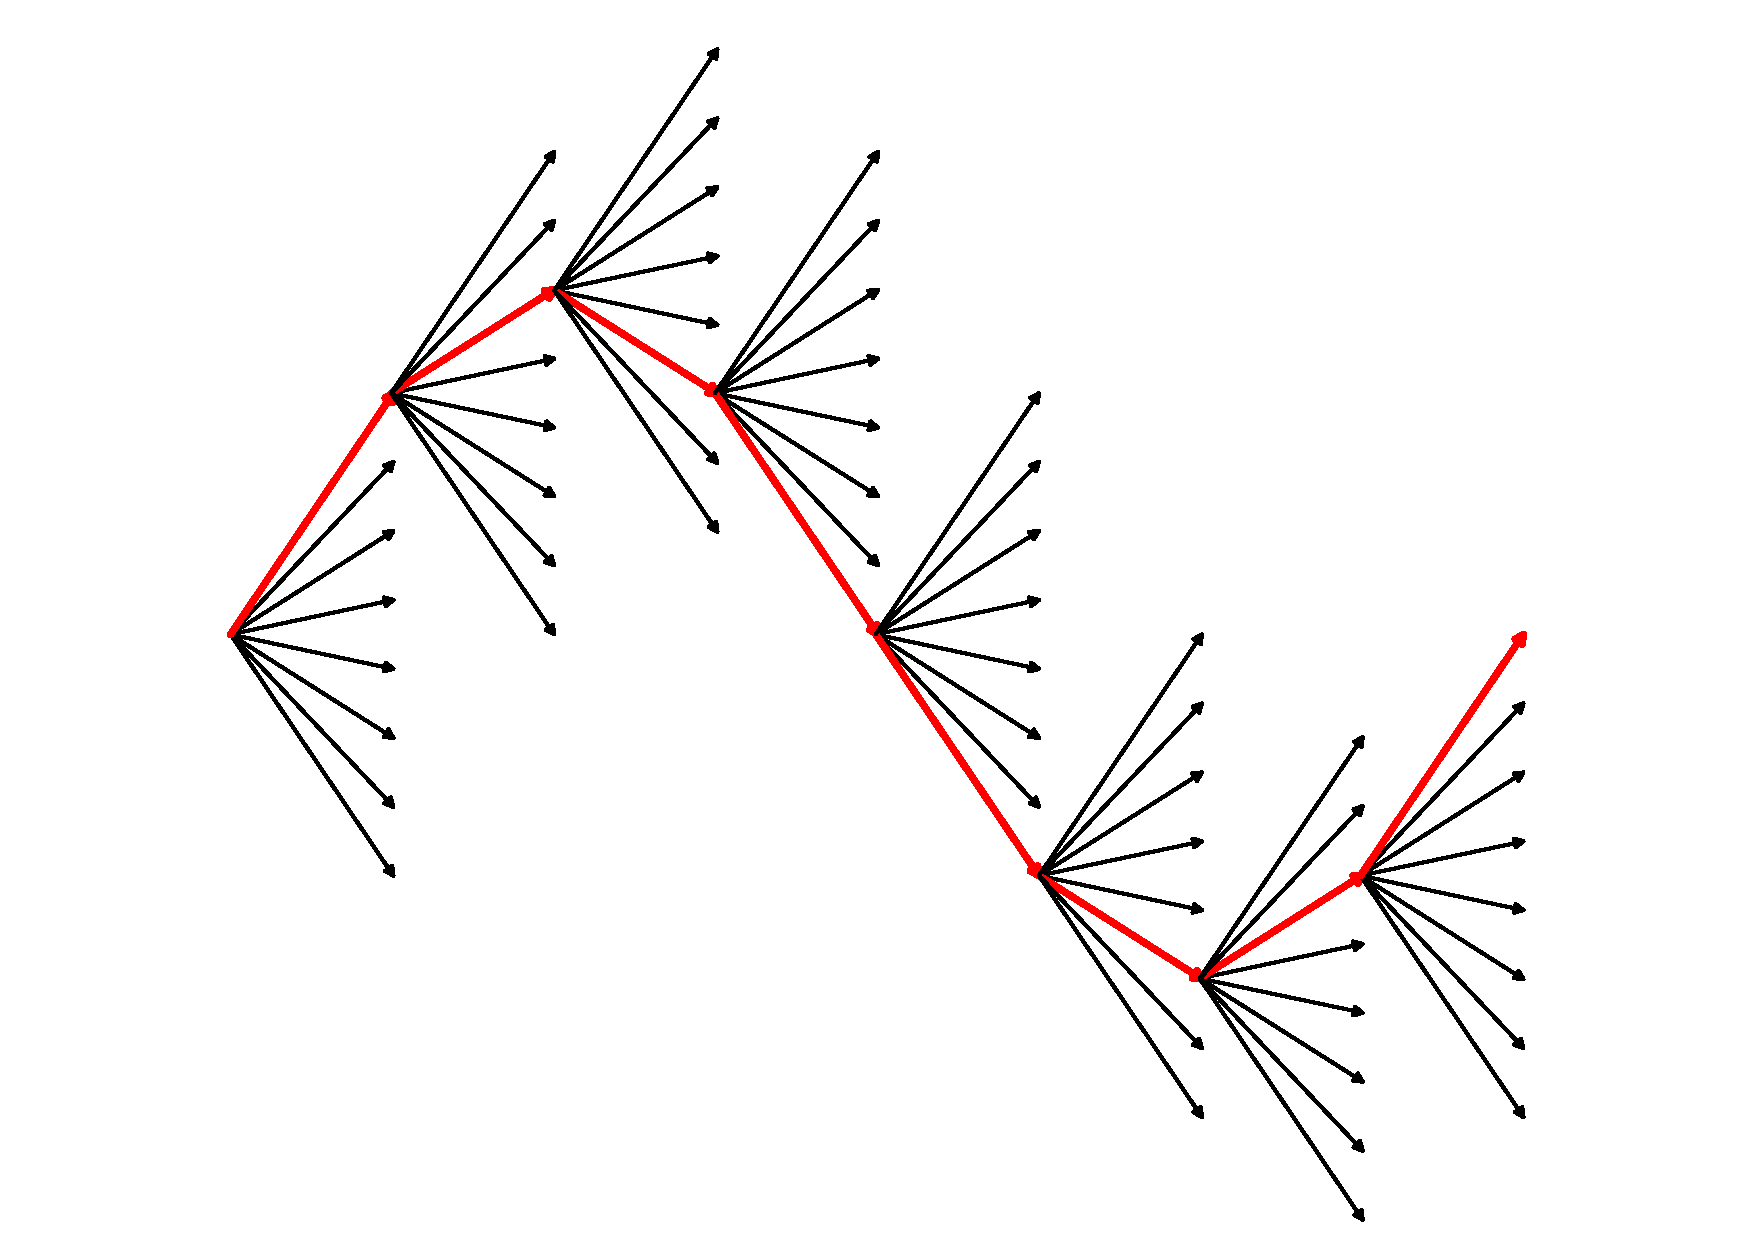
\includegraphics[width=0.75\textwidth]{RCgeneration_SineWave_byHand.pdf} %width=1
   \caption{Riemanncode generation for a sine wave by hand}
   \label{fig:SineWaveCodeGeneration}
\end{figure}

This generated Riemann code was used to synthesize some sine waves in the frequency range between \gls{ab:dc} and \SI{6}{\GHz}.

\begin{figure}[htb!]
   \centering
   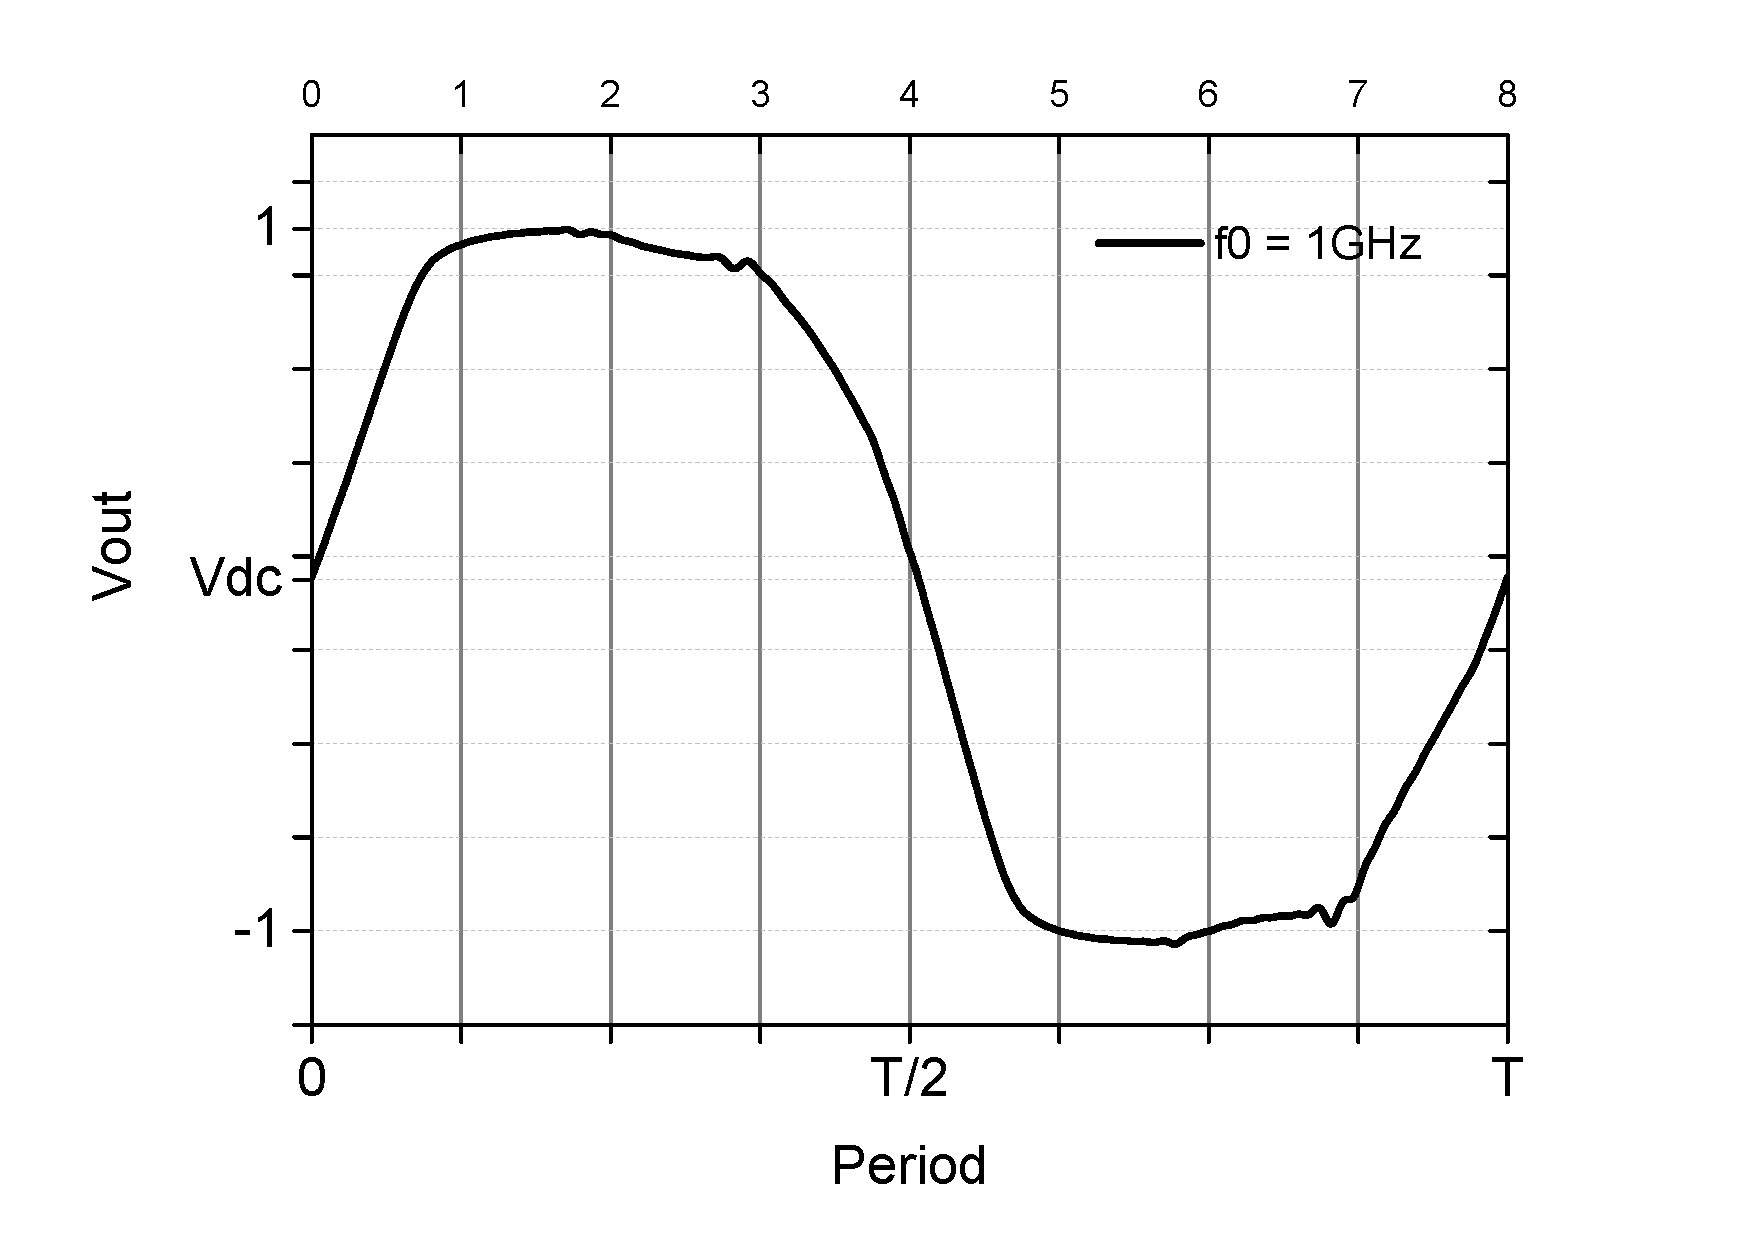
\includegraphics[width=0.75\textwidth]{Vout_sine_sampling_1GHz_1period.pdf}
   \caption{Synthesized signals}
   \label{fig:SynthesizedSignalWithStatedRiemanncode}
\end{figure}


\begin{figure}[htb!]
   \centering
   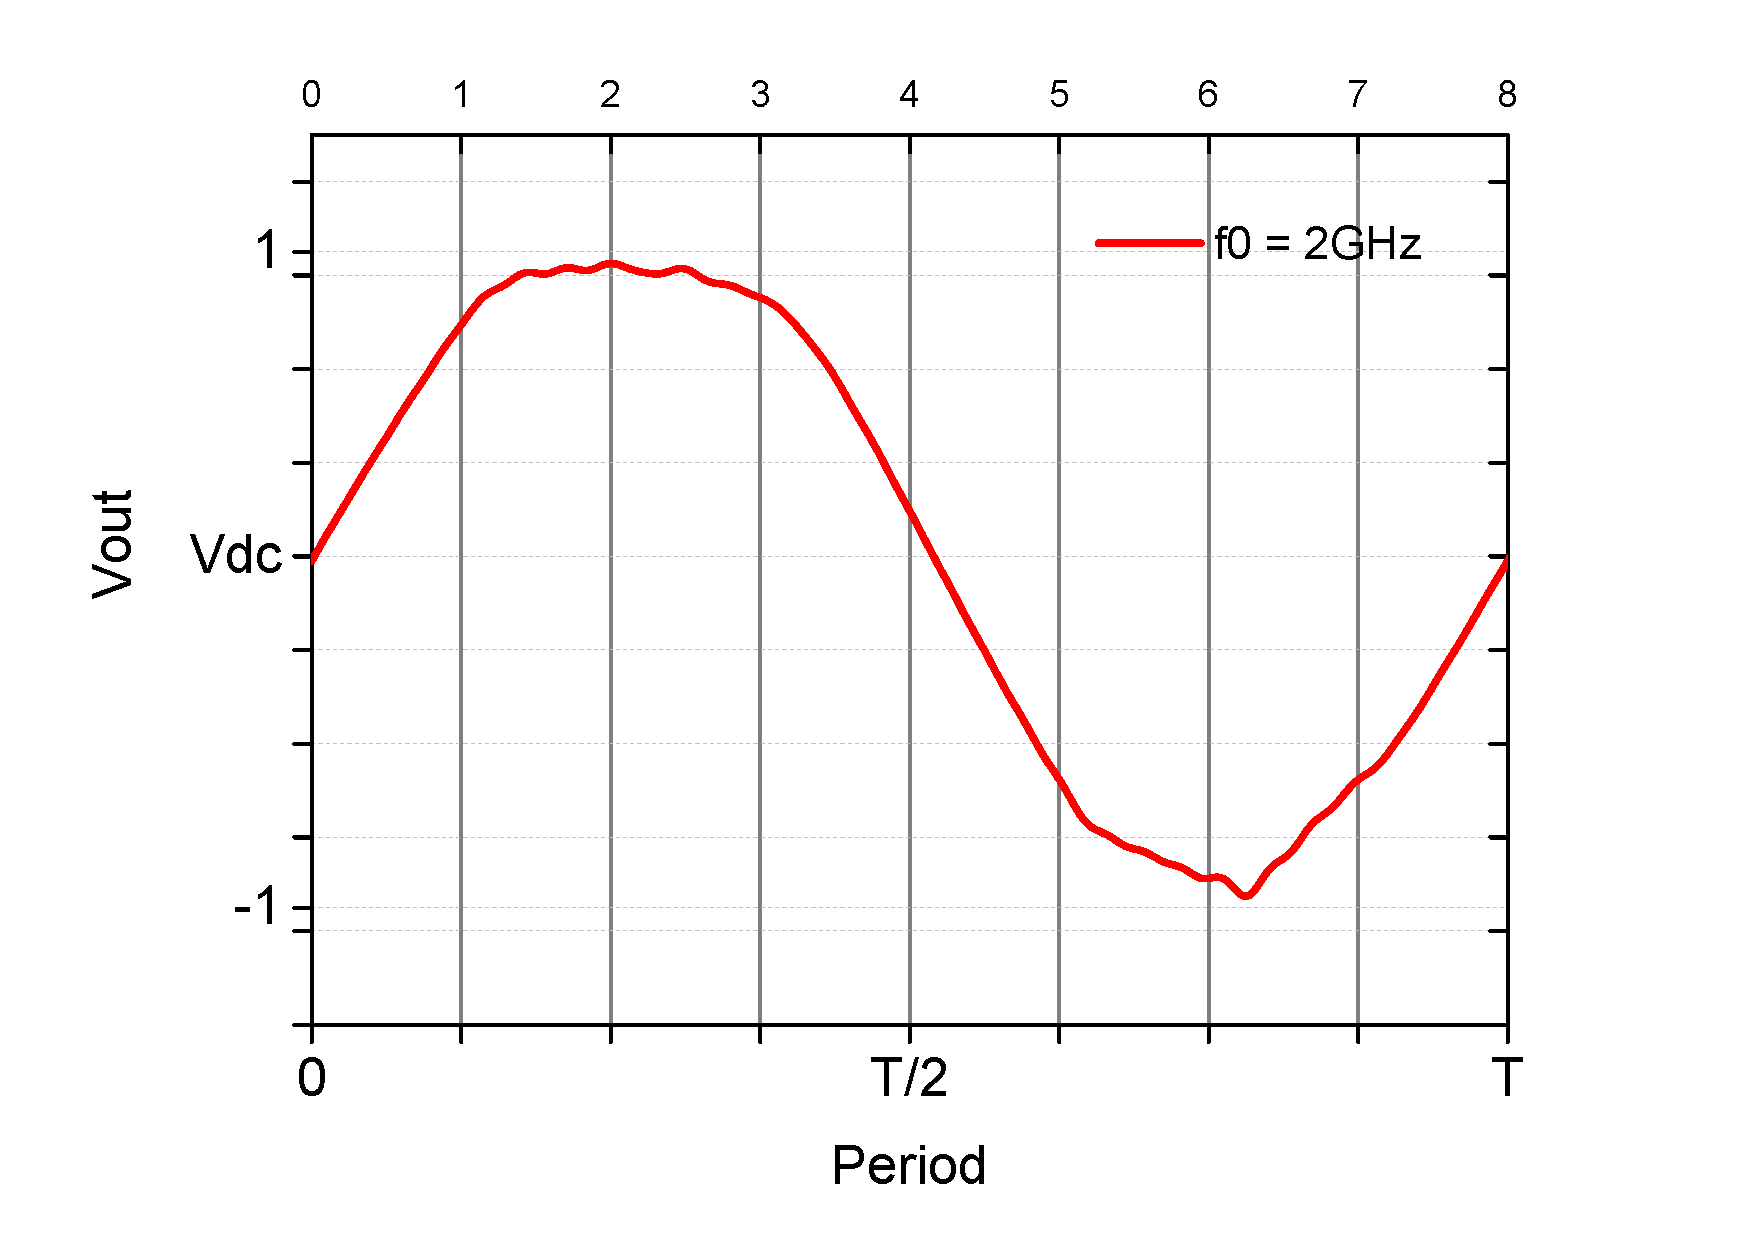
\includegraphics[width=0.75\textwidth]{Vout_sine_sampling_2GHz_1period.pdf}
   \caption{Synthesized signals}
   \label{fig:SynthesizedSignalWithStatedRiemanncode}
\end{figure}

%
%\begin{figure}
%\centering
%\begin{minipage}{.5\textwidth}
%  \centering
%  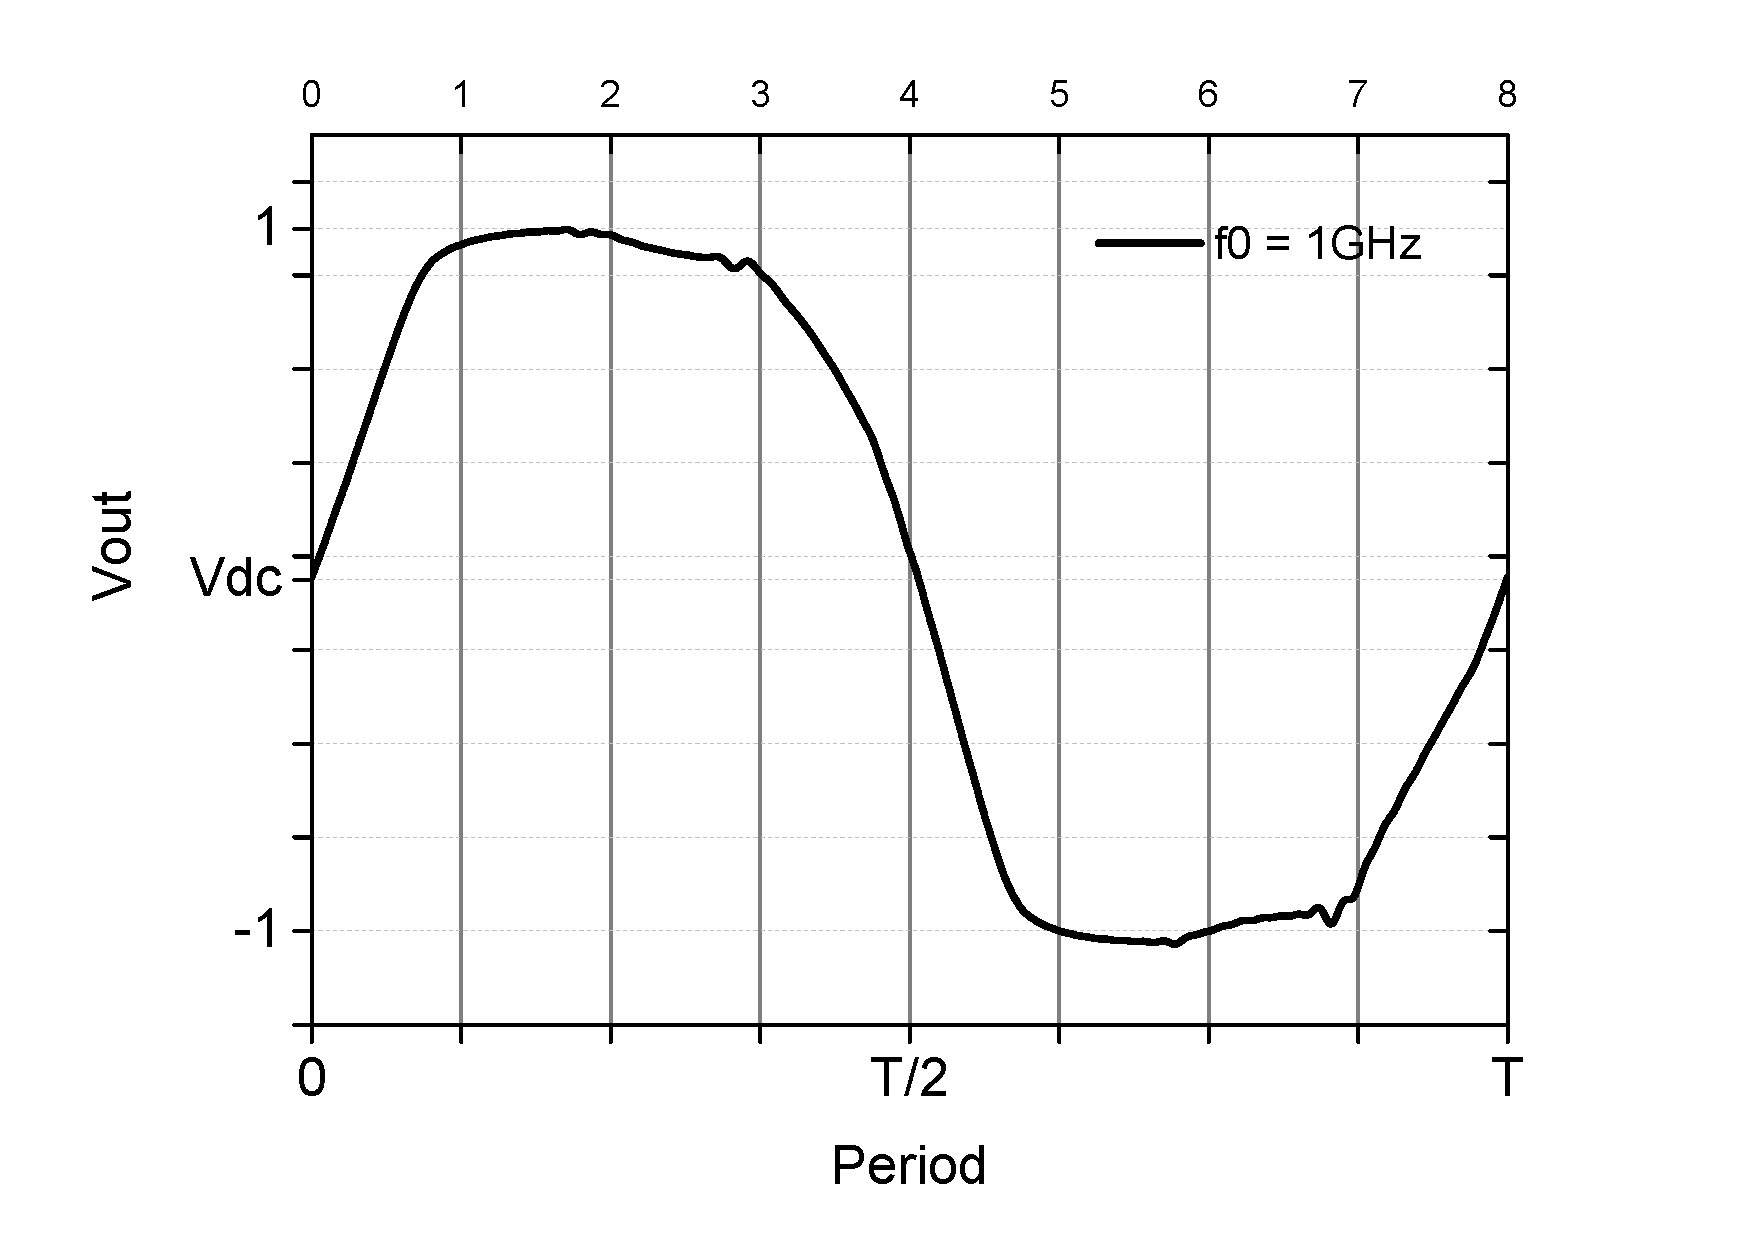
\includegraphics[width=1\linewidth]{Vout_sine_sampling_1GHz_1period.pdf}
%%  \captionof{figure}{A figure}
%  \label{fig:test1}
%\end{minipage}%
%\begin{minipage}{.5\textwidth}
%  \centering
%  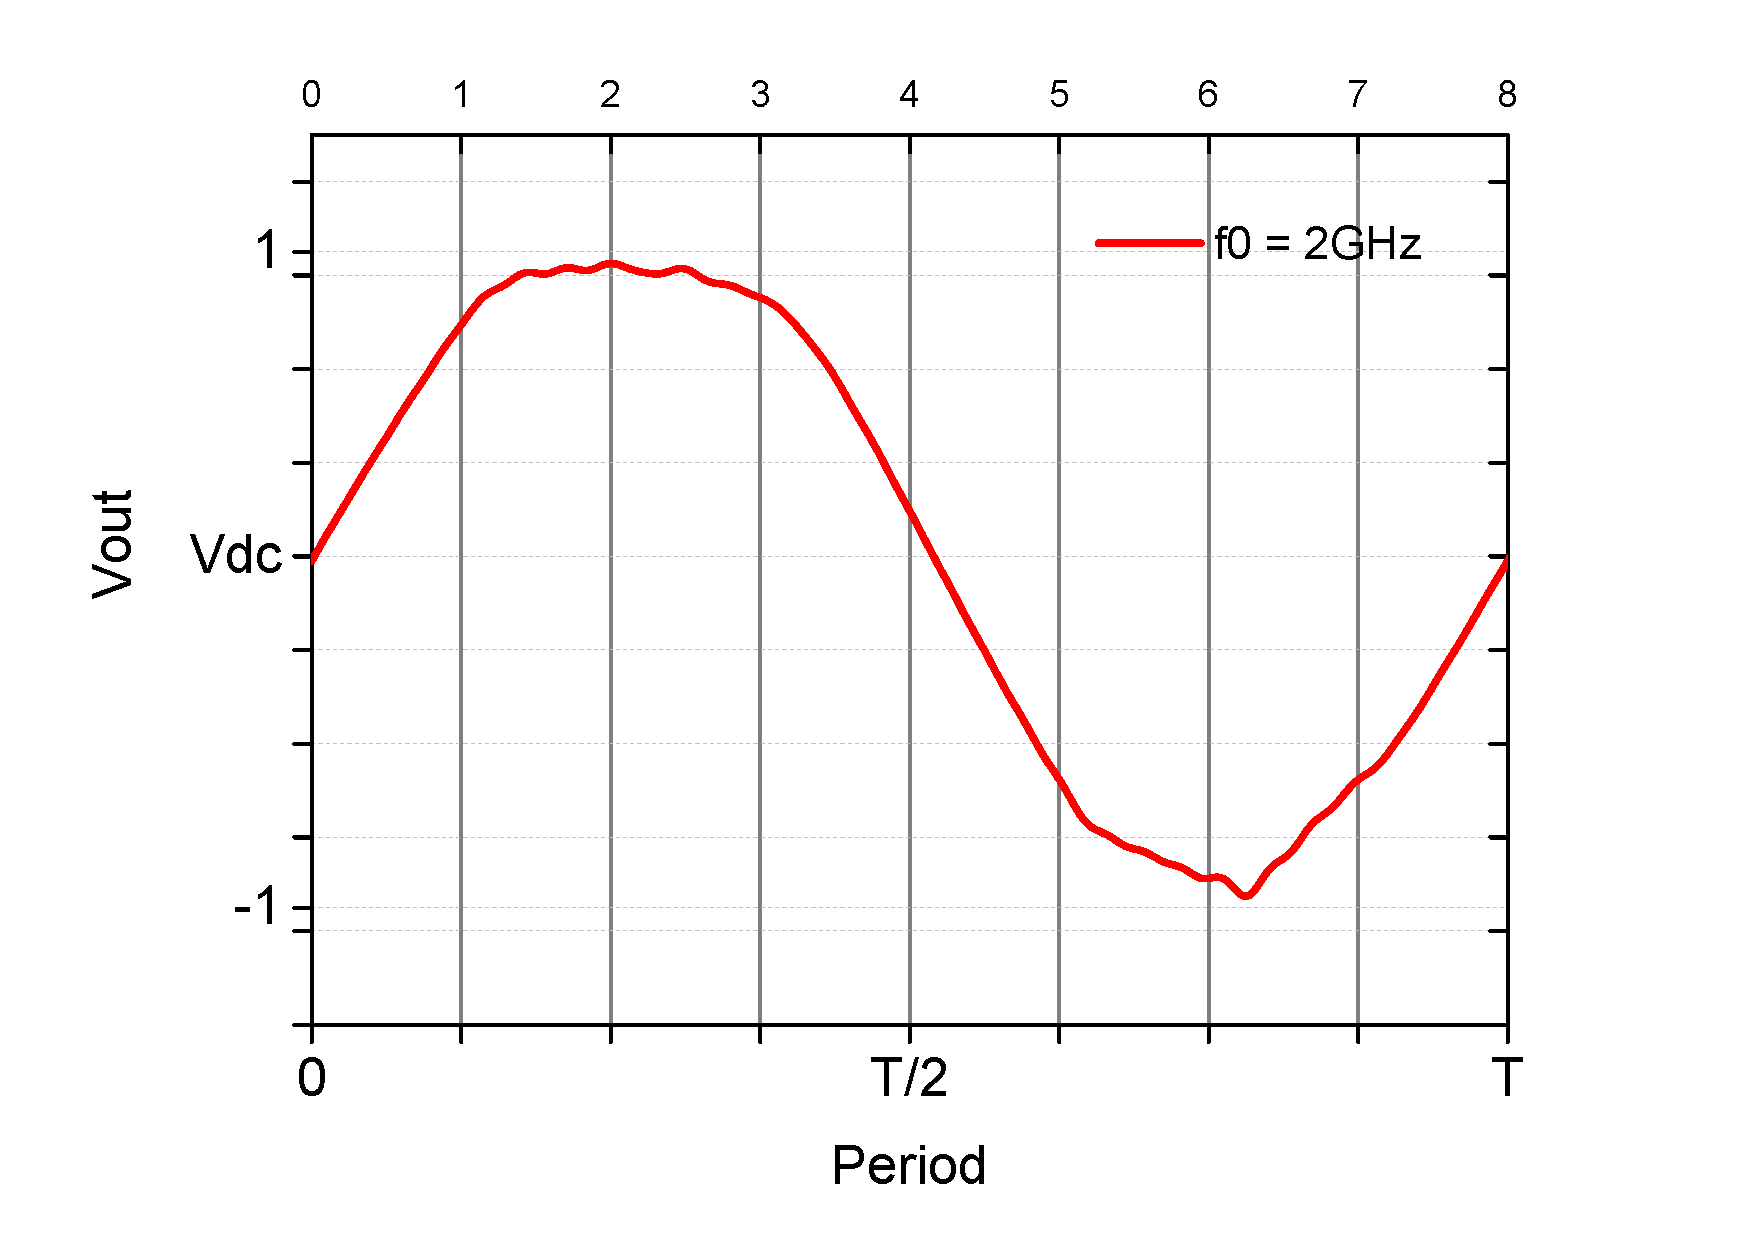
\includegraphics[width=1\linewidth]{Vout_sine_sampling_2GHz_1period.pdf}
%%  \captionof{figure}{Another figure}
%  \label{fig:test2}
%  \caption{Synthesized signal at \gls{sy:freq}= 1 GHz and 2 GHz with stated Riemann code}
%\end{minipage}
%\end{figure}
%















The time domain simulation of the output voltage in the Riemann Pump circuit exhibits the desired behaviour. 
As seen in Figure \ref{fig:SineWaveSynthVsTheoretical} a sine wave signal can be precisely synthesized. 
The sine wave is expressed as 
\begin{equation}
	v(t)= \widehat{v} \cdot sin( 2  \pi  f \cdot  t + \phi),
\end{equation}
with this parameters: $\widehat{v} = \SI{7.5}{\volt}$, $f = \SI{1}{\giga \hertz}$, $\phi = \pi / 4$.

\begin{figure}[htb!]
   \centering
   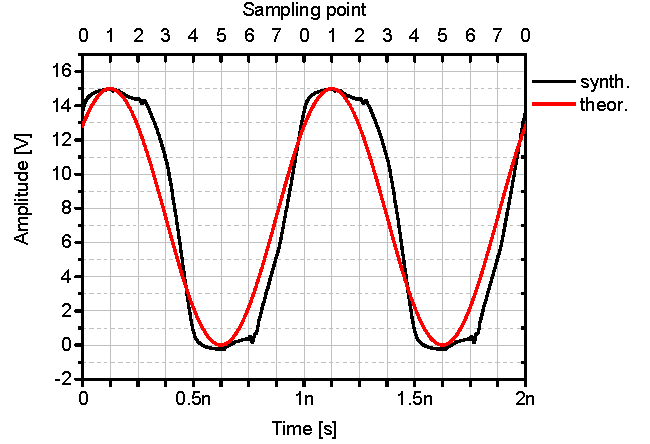
\includegraphics[width=0.75\textwidth]{Vout_SynthVsTheo.pdf}
   \caption{Synthesized sine wave with the theoretical sine wave}
   \label{fig:SineWaveSynthVsTheoretical}
\end{figure}

Although the fit seems to be very good, two distortions are visible. 

The deviation of the synthesized signal (black) from the desired one (red) is highlighted in Figure \ref{fig:SineCompare}.
Here the theoretical signal is presented in contrast to the synthesized one with their spectra.
% versus the synthesized signal is presented with their corresponding spectrum
The spectrum (Fourier transformation) demonstrates how accurate the signal is synthesized compared to the desired sine wave.\\
On the top left side the theoretical sine wave is plotted in red. Underneath of it the spectrum states a frequency portion for the direct component at \SI{0} {\GHz} and a fundamental frequency portion at \SI{1}{\GHz}.
This Fourier transformation represents the theoretic frequency portions of a clear sine wave. 
In comparison to this it seems that the synthesized signal on the top right side be a good approximation.
The spectrum on the bottom right side exhibits some distortion induced from the quantization process. 
Beside the direct component and the fundamental frequency component there are some other frequency portions which do not occur in the optimal sine wave spectrum.
The bottom right plot of Figure \ref{fig:SineCompare} shows that the distortion is maximal \SI{1}{\volt} in amplitude at a the third harmonic. The 2nd to 10th harmonic are at most a half of a volt.\\
\textit{The accuracy is very good. This can be verified by the signal to noise ratio -> explain, state the SNR}

\begin{figure}[htb!]
	\centering
  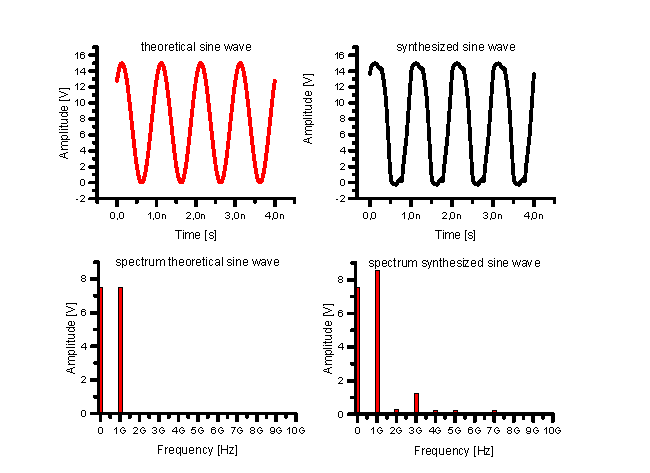
\includegraphics[width=1\textwidth]{SineCompare.pdf}
	\caption{Comparison between a theoretical and a synthesized sine wave with their spectrum}
	\label{fig:SineCompare}
\end{figure}

To address already some limitations (of this approach) which occurred during the simulation Figure \ref{fig:7SignalsSameSlopeInOnePlot} shows seven signals synthesized with the same digital Riemann code but different sampling rates.
The signals amplitude is plotted over the radian, representing two periods of the signal.
The plot over the radian makes it easier to compare the signals while they have different frequencies and hence periods.\\
The shapes of the signals with frequencies between \SI{2}{\GHz} and \SI{6}{\GHz} all nicely fit to the expected synthesized sine wave shape. Due to the different periods of sampling time the amplitude of each signal differs, hence the output capacitor is charged for different times.\\
The black and the blue signal with signal frequency \SI{1}{\GHz} and  \SI{500}{\MHz} respectively differ from the expected shape of a sine wave. While the black signal could represent a sine wave with a DC offset of 7.5Vdc and an amplitude of 7.5V the blue signal already shapes like a rectified sine signal. The blue signal which should represent a sine wave with a signal frequency of \SI{500}{\MHz} is clipped and hence shows the behaviour of a rectangular signal. This undesired behaviour is induced from a fully charged output capacitance. \\
The maximum amplitude for the capacitor is the supply voltage of \SI{15}{\volt}. If this maximum is reached, the signal wave form is clipped right there.


%For the baseband frequency of \SI{500}{\MHz} the sampling frequency is eight times baseband frequency due to \gls{ab:osr} and Nyquist-Shannon theorem.
%A sampling frequency of \SI{4} {\GHz} means a sampling time of \SI{250}{\pico \second}, hence the output capacitance is \SI{20}{\pico \farad} it is charged with  .


\begin{figure}[htb!]
   \centering
   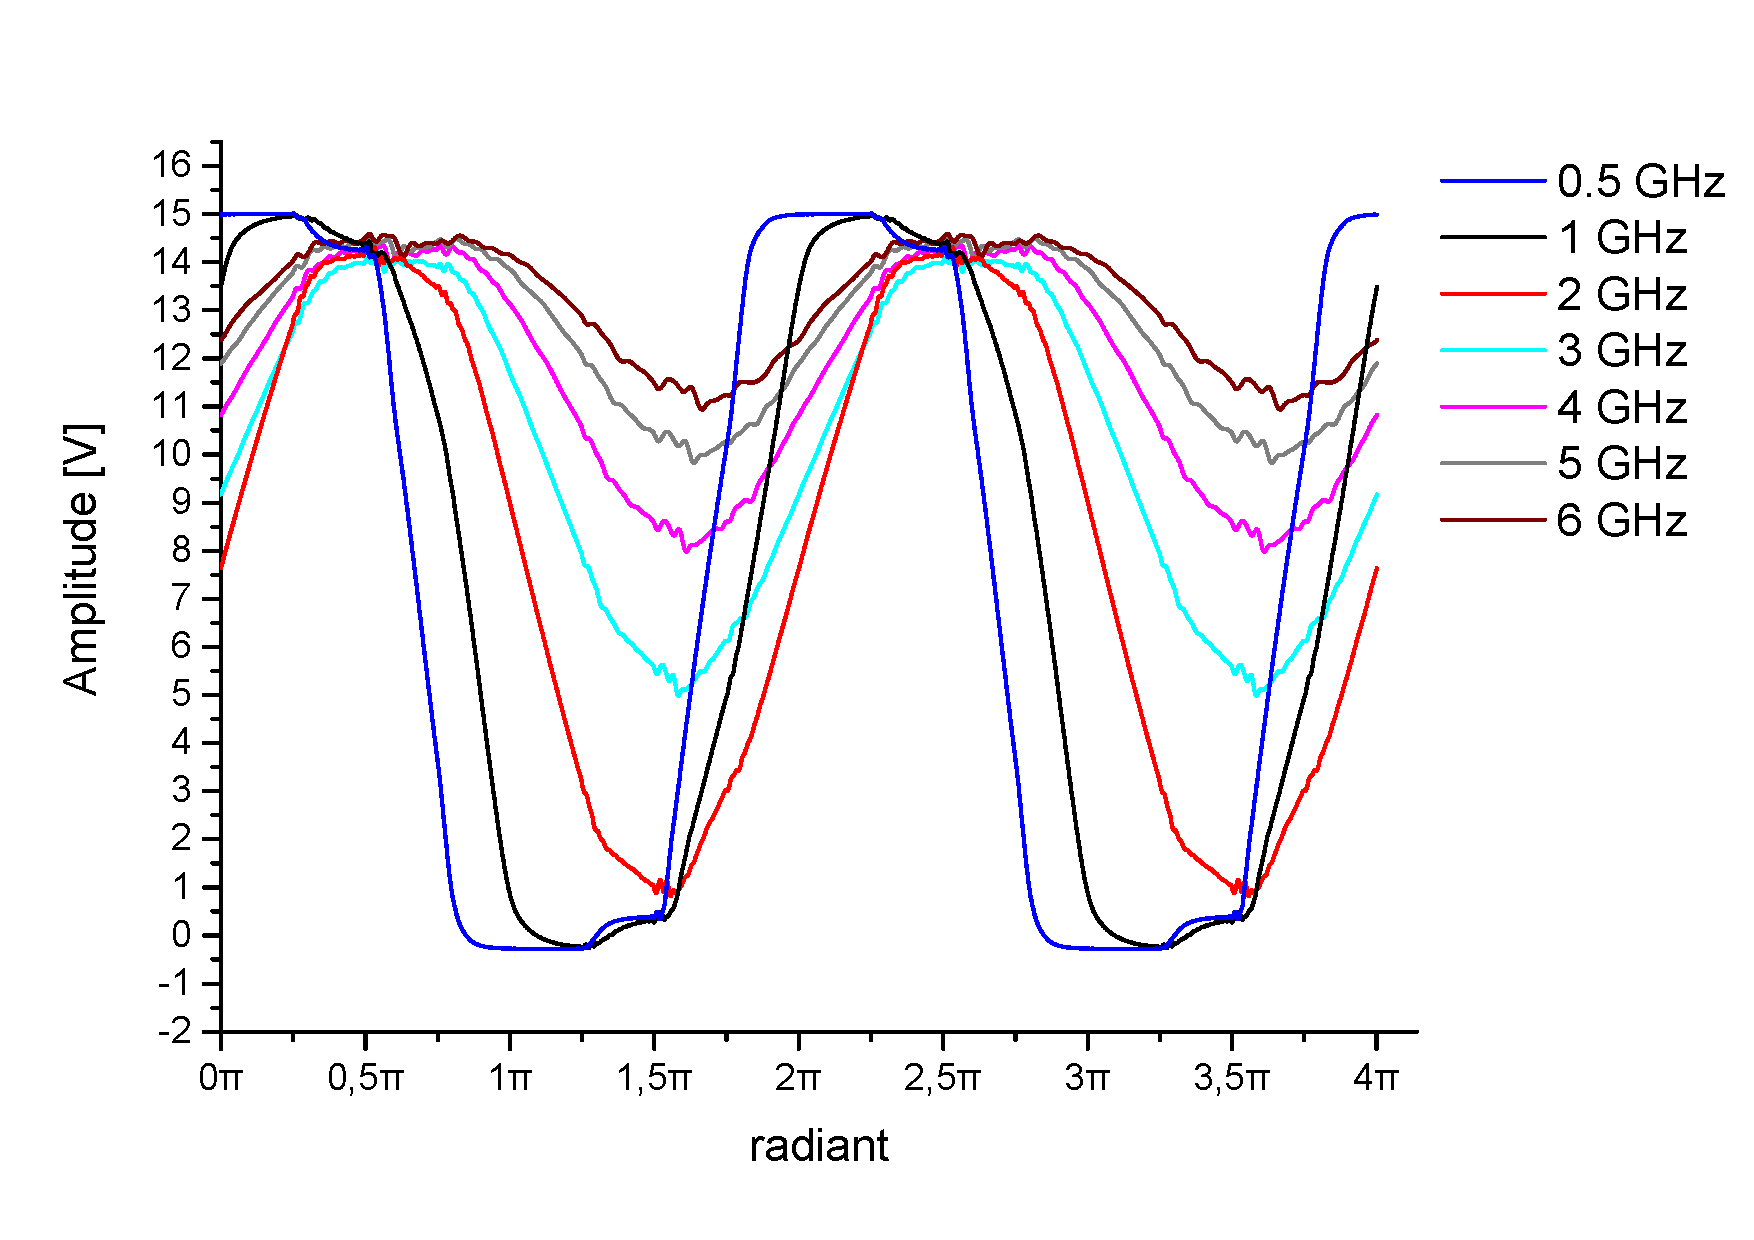
\includegraphics[width=0.75\textwidth]{Vout_sine_7signals_inOne_3bit_osr4.pdf}
   \caption{Signals synthesized with Riemann code introduced with Figure \ref{fig:SineWaveCodeGeneration}}
   \label{fig:7SignalsSameSlopeInOnePlot}
\end{figure}

\subsection{rectified sine wave generation in the time domain}
Based on the same optical approximation of the signal in Figure \ref{fig:SineWaveCodeGeneration} the riemanncode for the half sine is generated. The Riemanncode for the half sine is: 000 010 101 111 000 010 101 111
\subsection{triangular wave generation in the time domain}
This is a triangular wave.


\section{Stability analysis of the realised circuit}
The stability analysis is important to ensure that the circuit under test do not oscillate. 
 To check this, the complex impedance at specific points in the circuit is measured.
 If the real part of the impedance is positive for the whole frequency range of the simulation, it indicates in an easy way that the circuit does not oscillate.
This simulation is done within the ADS tool. 

\section{Energy consumption analysis of the realised circuit}
Due to the idea to use the presented topic for mobile communication it could be implemented in mobile devices, although this thesis only handles the device for the basestation. If it could be used in a mobile device the energy consumption is critical.\\
The energy consumption of the designed circuit in chapter \ref{ch:design} is simulated with \gls{ab:ads}.\\
 For the chips used for the demonstrator refer to the work of Stephan Maroldt who states, that the power consumption is:  divided into static and dynamic ones. The switching losses are greater than the static ones.
The losses are divided into dynamic losses of the switches and static losses.
% switch voltage for on/off state, switch time, static losses and dynamic losses.

\section{Proof of concept simulation with existing components}
This simulation is based on the measurements and the design of various chips from Stephan Maroldt.
This two bit resolution simulation is done to compare the demonstrators measurements with the simulation. \textbf{two-bit resolution, osr = 4, keep it small and simple, frequency higher, demonstrator, assembly, less complex} 
The three bit resolution DAC was too complex to realize in a first approach on a hybrid substrate. Therefore an easier approach was designed to validate the proof of concept.

\section{Evaluation of the simulation results for the Riemann Pump}
evaluate the simulation results, what is to expect in realisation. 
What is the expectation to the measurement?
